\subsection{Deconvolution}
\begin{frame}
  \frametitle{Simple adaptations}
  \begin{block}{PSF estimation}
    We need
    \begin{itemize}
      \item Pure blurred image;
      \item Not too small.
    \end{itemize}
    The biggest square of foreground seems good but not necessarily
    pure since it is an upper bound.

    Let's take the biggest square $-3$ pixels at each borders.
  \end{block}
  \begin{block}{Wiener}
    Deblur the subimage then only change pixels of the connected
    shape.
  \end{block}
\end{frame}

\begin{frame}
  \frametitle{``select-lucy''}
  \begin{block}{``select-lucy''}
    Since it is iterative, we can do better than Wiener.
    At \emph{each} iteration, only change pixels of the connected
    shape.
  \end{block}
  \begin{myfig}{select-lucy-zooms}{Zoom on ``select-lucy'' solution.}
    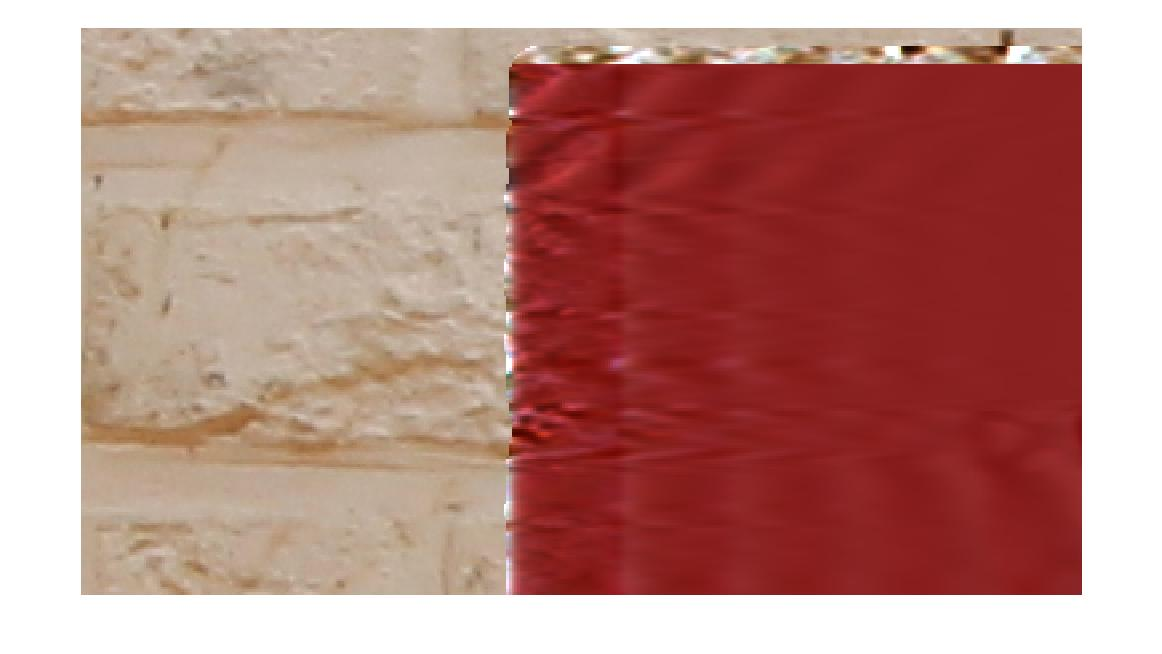
\includegraphics[height=5cm]{dontpanic-40-0_2_1-100_zoom.jpg}
  \end{myfig}
\end{frame}

\begin{frame}[allowframebreaks]
  \frametitle{``exact-lucy''}
  \myfullfig{car-middlediff}{Plot of the diff (foreground $-$ background normalized by variance)}{0.5}
  \begin{block}{``exact-lucy''}
    Absolute value of the slope of the linear regression of $L$ consecutive diffs
    maximized at start and end of background.

    \begin{enumerate}
      \item Estimate the ``exact'' foreground.
      \item Blur it and get an estimate of the ratio of background
        for each pixel.
      \item Remove the background.
      \item Use our modified iteration not sensible to black.
    \end{enumerate}
  \end{block}
  \begin{myfig}{exact-lucy-zooms}{Zoom on ``exact-lucy'' solution.}
    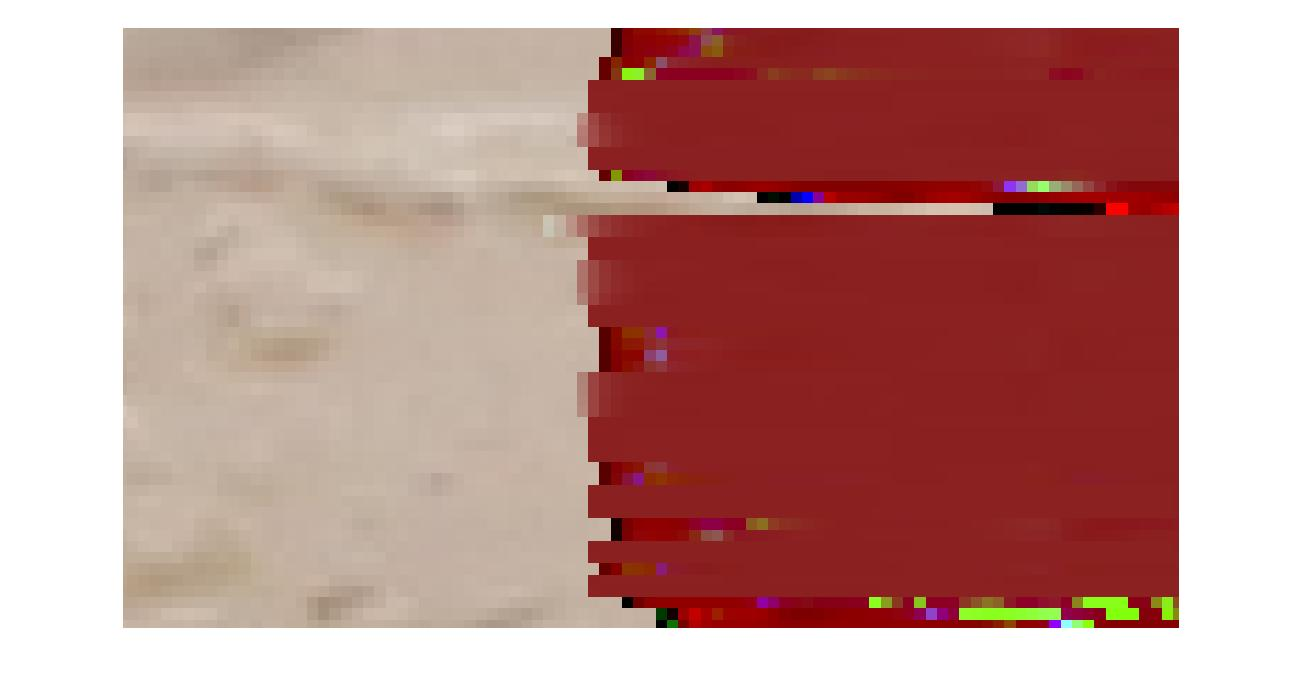
\includegraphics[height=5cm]{dontpanic-40_0-2_2-100_zoom.jpg}
  \end{myfig}
  \begin{block}{Conclusion}
    Lucy-Richardson likes degrees of freedom (recall ``magic-lucy'' success).
  \end{block}
\end{frame}
